% !TeX root = ../main.tex

\chapter{Figures, Tables, and Equations}

This chapter is a compact writing guide for common analysis-note material. It
can be removed from a production note after the real chapters are in place.

\section{Figures}

Use \env{figure} for single figures and \env{subfigure} for panel figures. Keep
analysis plot files under \file{figures/} when possible.

\begin{figure}[htbp]
  \centering
  
\includegraphics[width=0.28\textwidth]{STAR-logo-base-red.pdf}
  \caption{Single-figure example. Replace the logo with an analysis plot.}
  \label{fig:single-example}
\end{figure}

Figure~\ref{fig:single-example} shows the recommended basic structure: center
the graphic, write a complete caption, and place \cs{label} immediately after
\cs{caption}.

\begin{figure}[htbp]
  \centering
  \begin{subfigure}{0.47\textwidth}
    \centering
    
\includegraphics[width=0.58\linewidth]{STAR-logo-base-red.pdf}
    \caption{Main STAR logo}
    \label{fig:star-logo-red}
  \end{subfigure}
  \hfill
  \begin{subfigure}{0.47\textwidth}
    \centering
    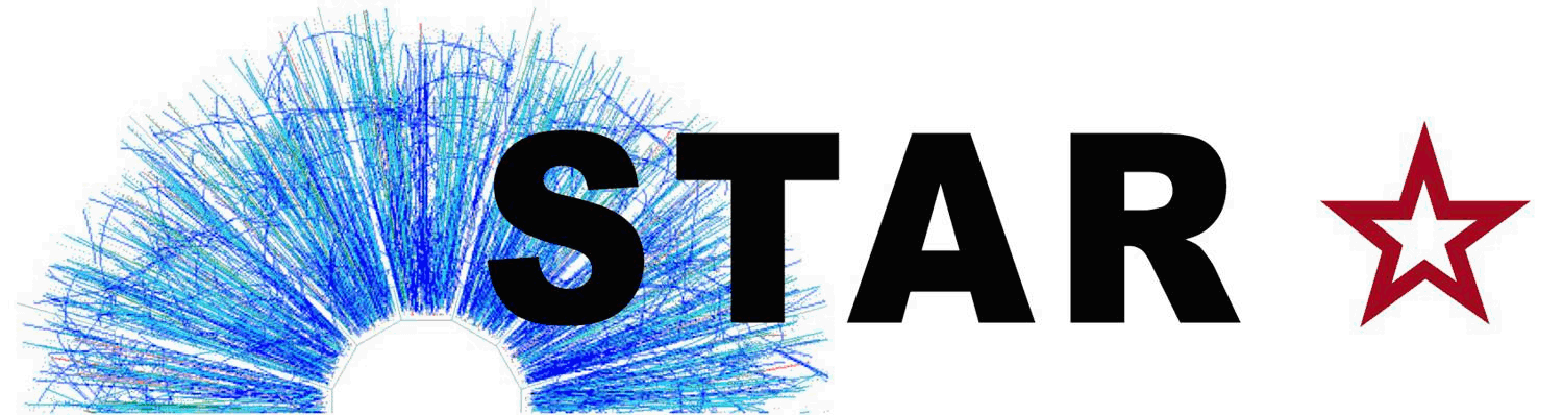
\includegraphics[width=0.58\linewidth]{STAR-logo-trans.pdf}
    \caption{Transparent STAR logo}
    \label{fig:star-logo-transparent}
  \end{subfigure}
  \caption{Two-panel figure example using the \pkg{subcaption} package.}
  \label{fig:pair-panels}
\end{figure}

\section{Tables}

Use \pkg{booktabs} for publication-style tables and avoid vertical rules. For
numbers with aligned uncertainties, use \pkg{siunitx}.

\begin{table}[htbp]
  \centering
  \caption{Event and track selection example.}
  \label{tab:selection-example}
  \begin{tabular}{lll}
    \toprule
    Category & Requirement & Purpose \\
    \midrule
    Event vertex & $|V_{z}| < \SI{30}{cm}$ & uniform acceptance \\
    Track quality & $n_{\mathrm{HitsFit}} > 20$ & stable momentum fit \\
    Kinematics & $p_{\mathrm{T}} > \SI{0.2}{GeV}/c$ & analysis phase space \\
    \bottomrule
  \end{tabular}
\end{table}

\begin{table}[htbp]
  \centering
  \caption{Example table with aligned numerical columns and table notes.}
  \label{tab:yield-example}
  \begin{threeparttable}
    \begin{tabular}{lS[table-format=3.0]S[table-format=2.1]S[table-format=1.3]}
      \toprule
      Centrality & {Raw yield} & {Efficiency (\%)} & {$R_{\mathrm{AA}}$} \\
      \midrule
      0--10\%  & 125 & 18.4 & 0.612 \\
      10--40\% & 248 & 22.7 & 0.731 \\
      40--80\% & 310 & 28.9 & 0.905 \\
      \bottomrule
    \end{tabular}
    \begin{tablenotes}
      \footnotesize
      \item Values are placeholders for demonstrating table formatting.
    \end{tablenotes}
  \end{threeparttable}
\end{table}

\section{Equations}

Use \env{equation} for single numbered equations and \env{align} when several
related expressions should align at relation symbols.

\begin{equation}
  R_{\mathrm{AA}}(p_{\mathrm{T}}) =
  \frac{1}{\langle N_{\mathrm{coll}}\rangle}
  \frac{\mathrm{d}^{2}N_{\mathrm{AA}}/\mathrm{d}p_{\mathrm{T}}\mathrm{d}y}
       {\mathrm{d}^{2}N_{pp}/\mathrm{d}p_{\mathrm{T}}\mathrm{d}y}.
  \label{eq:raa-definition}
\end{equation}

Equation~\ref{eq:raa-definition} is written without project-specific shortcut
commands. If you prefer shorthands such as \cs{pT}, define them in
\file{usercommands.tex}.

\begin{align}
  N_{\mathrm{sig}} &= N_{\mathrm{US}} - 2\sqrt{N_{++}N_{--}}, \\
  \sigma_{\mathrm{sig}}^{2} &= \sigma_{\mathrm{US}}^{2}
    + \frac{N_{--}}{N_{++}}\sigma_{++}^{2}
    + \frac{N_{++}}{N_{--}}\sigma_{--}^{2}.
  \label{eq:like-sign-subtraction}
\end{align}

Long formulae should be broken across lines before they become difficult to
read. Put short explanatory text outside the math environment.

\section{Algorithms}

For short procedural descriptions, \pkg{algorithm2e} is available. Use it only
when the procedure is clearer as steps than as prose.

\begin{algorithm}[htbp]
  \caption{Minimal correction workflow}
  \label{alg:correction-example}
  \KwIn{Raw signal yield $N_{\mathrm{raw}}$ and efficiency $\epsilon$}
  \KwOut{Corrected yield $N_{\mathrm{corr}}$}
  subtract residual background from $N_{\mathrm{raw}}$\;
  evaluate efficiency $\epsilon$ in the same kinematic interval\;
  compute $N_{\mathrm{corr}} = N_{\mathrm{raw}} / \epsilon$\;
\end{algorithm}
